\section{Introduction}

This \cgal\ component implements methods to analyze and process unorganized point sets.
The input is an unorganized point set, possibly with attributes such as unoriented or oriented normals.
This point set can be analyzed to measure common statistics quantities and bounding volumes such as average spacing, centroid, bounding box and bounding sphere.
We can furthermore process the point set with functions devoted to simplification, outlier removal, smoothing, normal estimation and normal orientation.
The output is a point set with normals.

% Insert image introduction.jpg/eps
\begin{center}
    \label{Point_set_processing_3-fig-introduction}
    % Image
    \begin{ccTexOnly}
        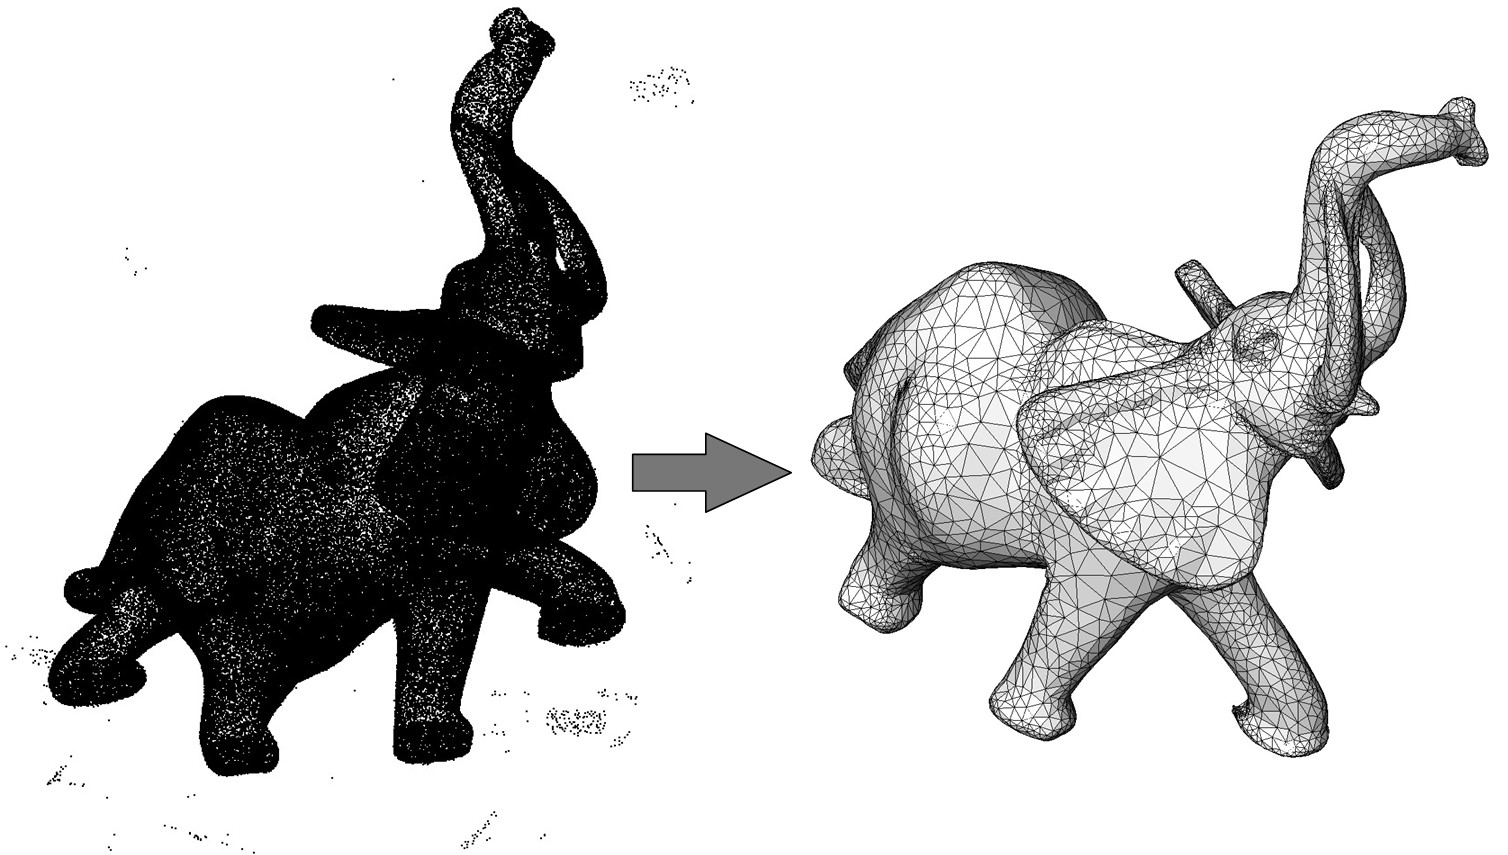
\includegraphics[width=1.0\textwidth]{Point_set_processing_3/introduction} % omit .eps suffix
    \end{ccTexOnly}
    \begin{ccHtmlOnly}
        <img width="90%" border=0 src="./introduction.jpg"><P>
    \end{ccHtmlOnly}
    % Title
    \begin{figure}[h]
        \caption{Point set processing.
                 Left: 4.4M points sampled on an elephant with a Minolta laser scanner.
                 Right: point set cleaned and simplified to 275K points.}
    \end{figure}
\end{center}


